\section{Anwendungsbeispiel}\label{kapitel8}
Den Benutzung von Gh0strunner werden wir in diesem Kapitel an einem Beispiel erklären. Unser Protagonist Eugen benutzt die App dabei zum ersten Mal.

\begin{figure}
\centering
\begin{minipage}{.4\textwidth}
  \centering
  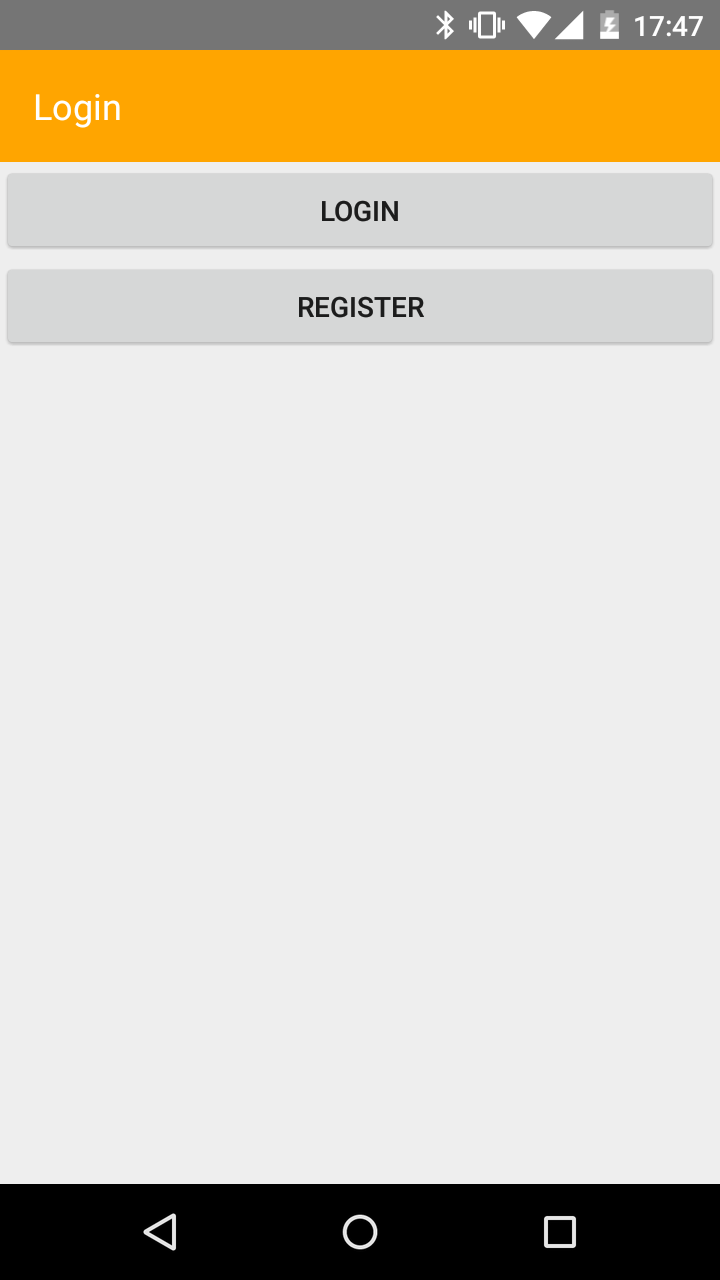
\includegraphics[width=.8\linewidth]{abb/bsp/bsp1}
  \captionof{figure}{Login Bildschirm}
  \label{fig:bsp1}
\end{minipage}%
\begin{minipage}{.4\textwidth}
  \centering
  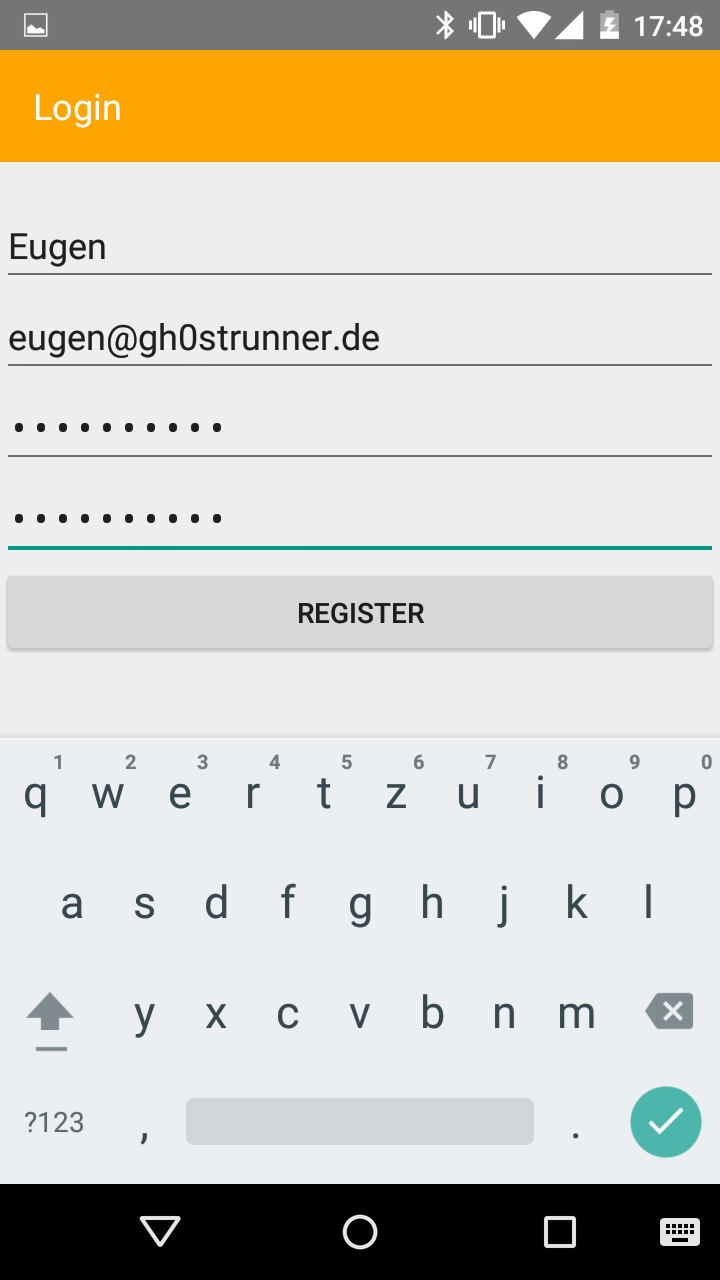
\includegraphics[width=.8\linewidth]{abb/bsp/bsp2}
  \captionof{figure}{Registrierung}
  \label{fig:bsp2}
\end{minipage}
\end{figure}

Als Eugen die App öffnet, sieht er, dass er sich zunächst anmelden oder registrieren muss.\ref{fig:bsp1} Da er noch kein Gh0strunner Konto besitzt, wählt er die \textit{Register} Option. \ref{fig:bsp2}

\begin{figure}
\centering
\begin{minipage}{.4\textwidth}
  \centering
  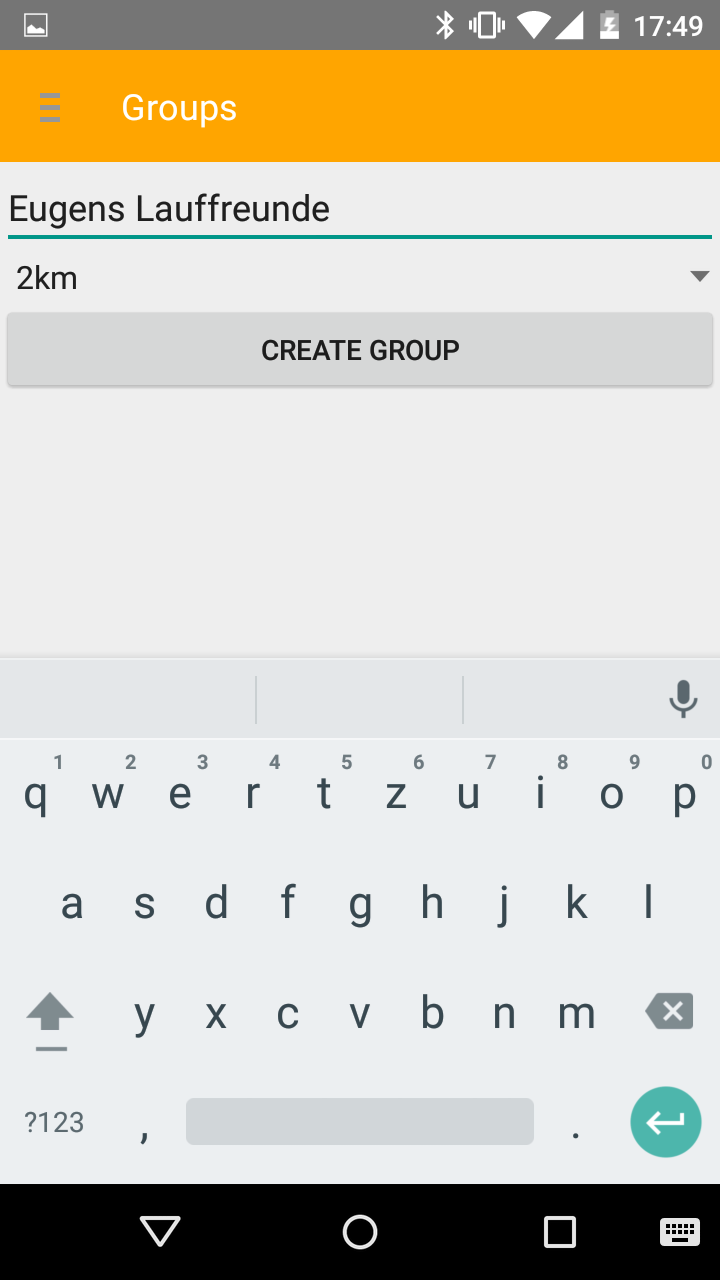
\includegraphics[width=.8\linewidth]{abb/bsp/bsp3}
  \captionof{figure}{Gruppe erstellen}
  \label{fig:bsp3}
\end{minipage}%
\begin{minipage}{.4\textwidth}
  \centering
  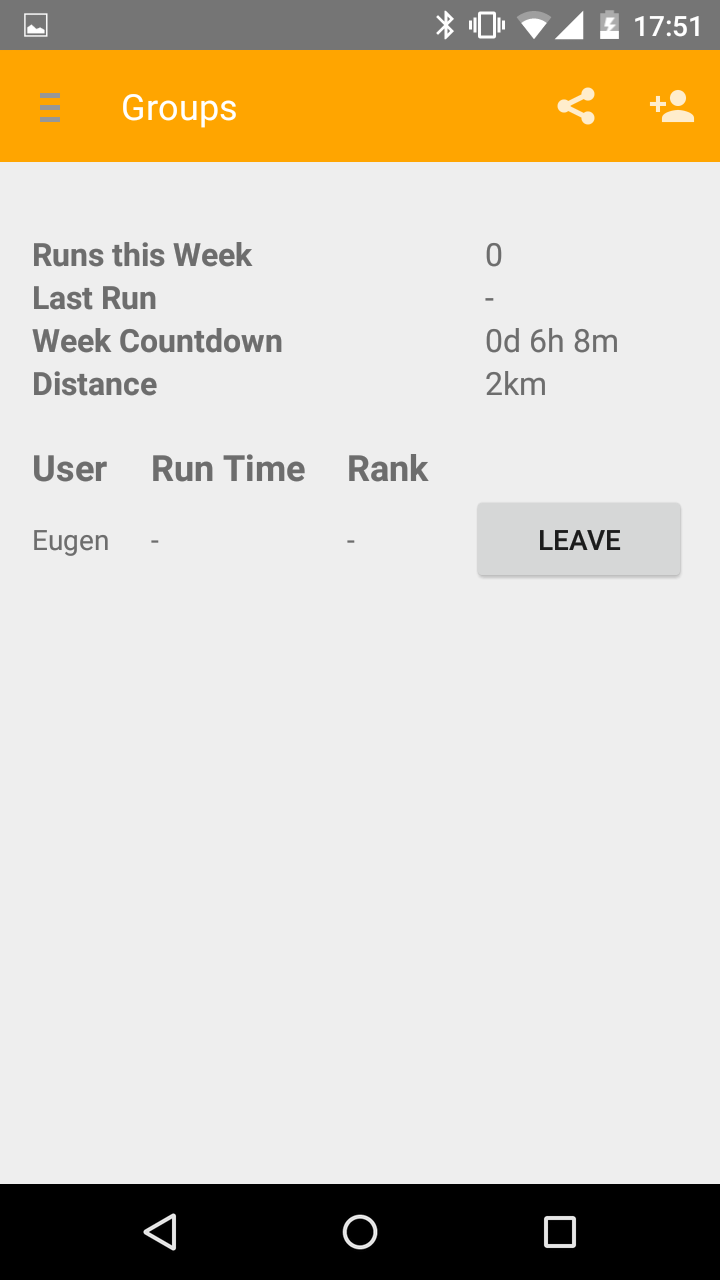
\includegraphics[width=.8\linewidth]{abb/bsp/bsp4}
  \captionof{figure}{Gruppenansicht}
  \label{fig:bsp4}
\end{minipage}
\end{figure}

Um später gegen seine Freunde antreten zu können, erstellt Eugen eine neue Gruppe. Eugen ist zwar sehr sportlich, weil er regelmäßig mithilfe der App GymWatch im Fitnessstudio trainiert, hat aber erst wenig Erfahrung mit Ausdauersport gesammelt. Deshalb entscheidet er sich in der neuen Gruppe für die kleinste Lauflänge von 2km. \ref{fig:bsp3} Anfangs ist Eugenleider das einzige Mitglied. \ref{fig:bsp4} 

\begin{figure}
\centering
\begin{minipage}{.4\textwidth}
  \centering
  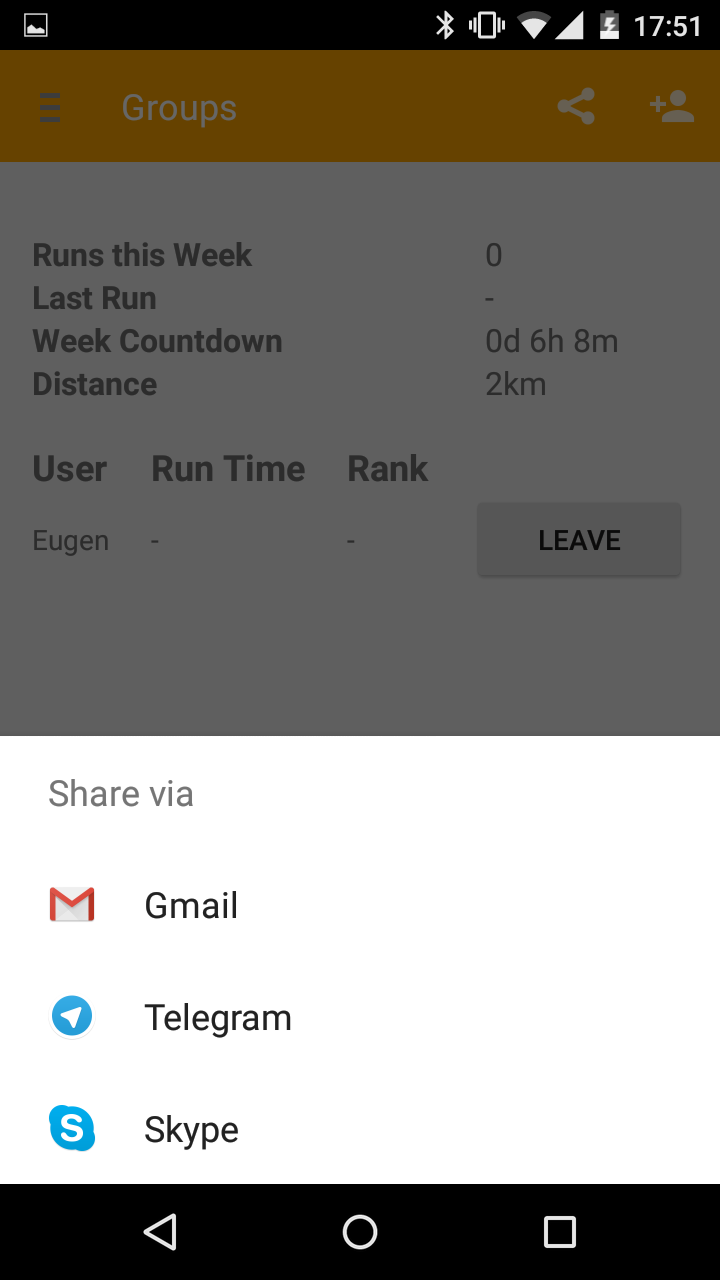
\includegraphics[width=.8\linewidth]{abb/bsp/bsp5}
  \captionof{figure}{Externe Einladung}
  \label{fig:bsp5}
\end{minipage}
\begin{minipage}{.4\textwidth}
  \centering
  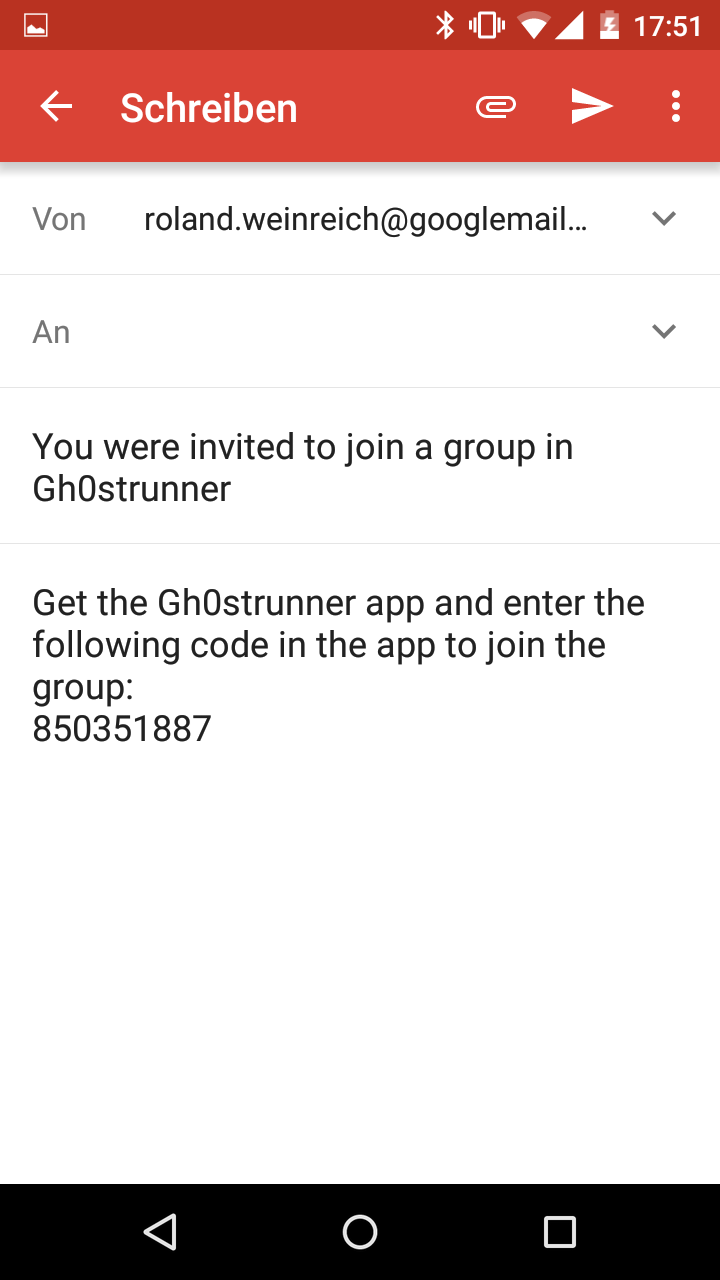
\includegraphics[width=.8\linewidth]{abb/bsp/bsp6}
  \captionof{figure}{Einladungstext als Email}
  \label{fig:bsp6}
\end{minipage}
\end{figure}

Er fühlt sich etwas einsam, deshalb lädt er seine gute Freundin Elena ein, die ebenfalls an einer Laufapp Interesse, aber noch nichts von Gh0strunner gehört hat. Dazu nutzt er die \textit{Teilen} Funktion der App. Mithilfe des erstellten Pincodes kann Elena später direkt der Gruppe beitreten. \ref{fig:bsp5} \ref{fig:bsp6}

\begin{figure}
\centering
\begin{minipage}{.4\textwidth}
  \centering
  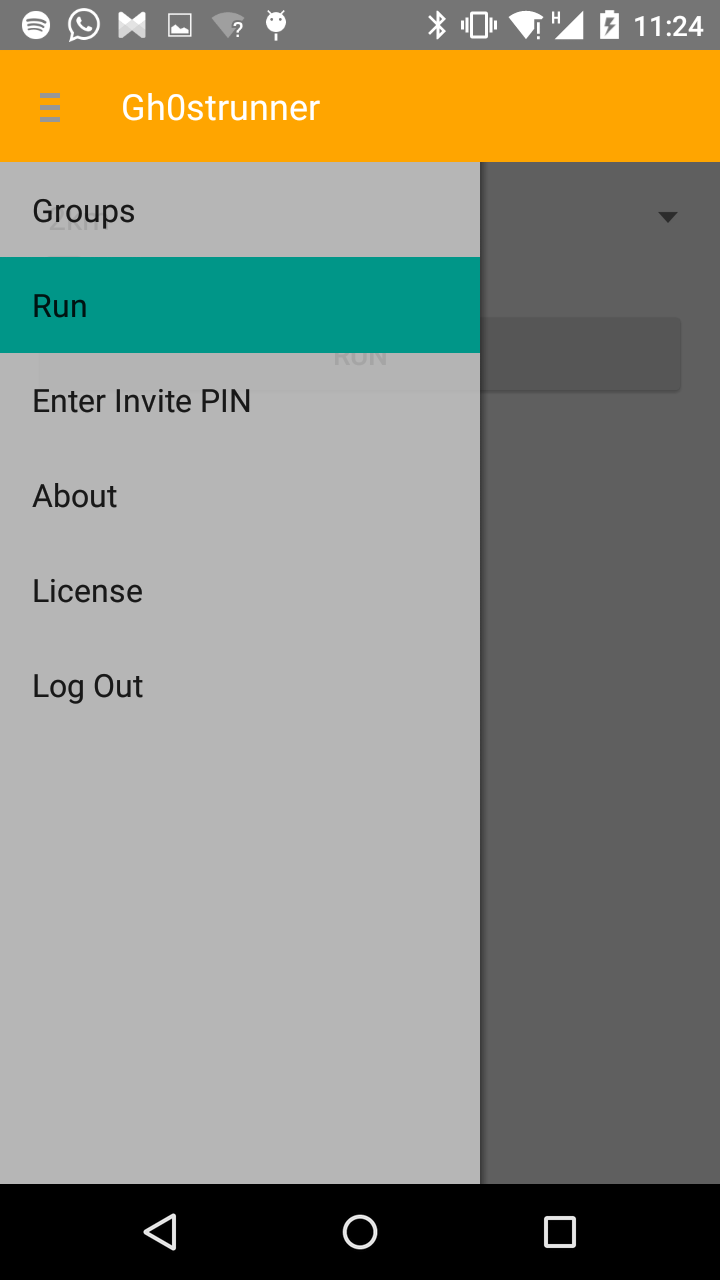
\includegraphics[width=.8\linewidth]{abb/bsp/bsp7}
  \captionof{figure}{Hauptmenü}
  \label{fig:bsp7}
\end{minipage}
\begin{minipage}{.4\textwidth}
  \centering
  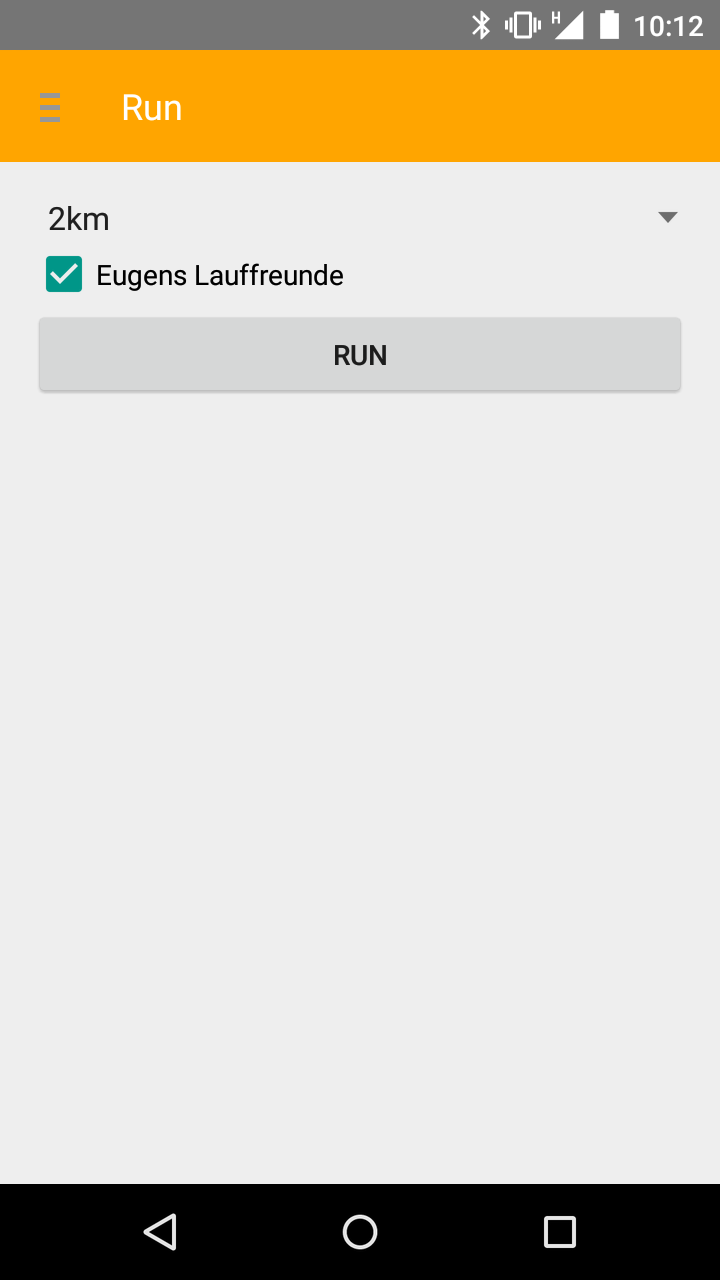
\includegraphics[width=.8\linewidth]{abb/bsp/bsp8}
  \captionof{figure}{Laufkonfiguration}
  \label{fig:bsp8}
\end{minipage}
\end{figure}

Nachdem er Elena eingeladen hat, entscheidet sich Eugen direkt seinen ersten Lauf zu starten. Die Option erreicht er über das seitlich aufklappbare Hauptmenü. \ref{fig:bsp7} Im Laufkonfigurationsmenü \ref{fig:bsp8} wählt er eine Lauflänge von  2 Kilometern, um den Lauf in der eben erstellten Gruppe hochladen zu können.

\begin{figure}
\centering
\begin{minipage}{.4\textwidth}
  \centering
  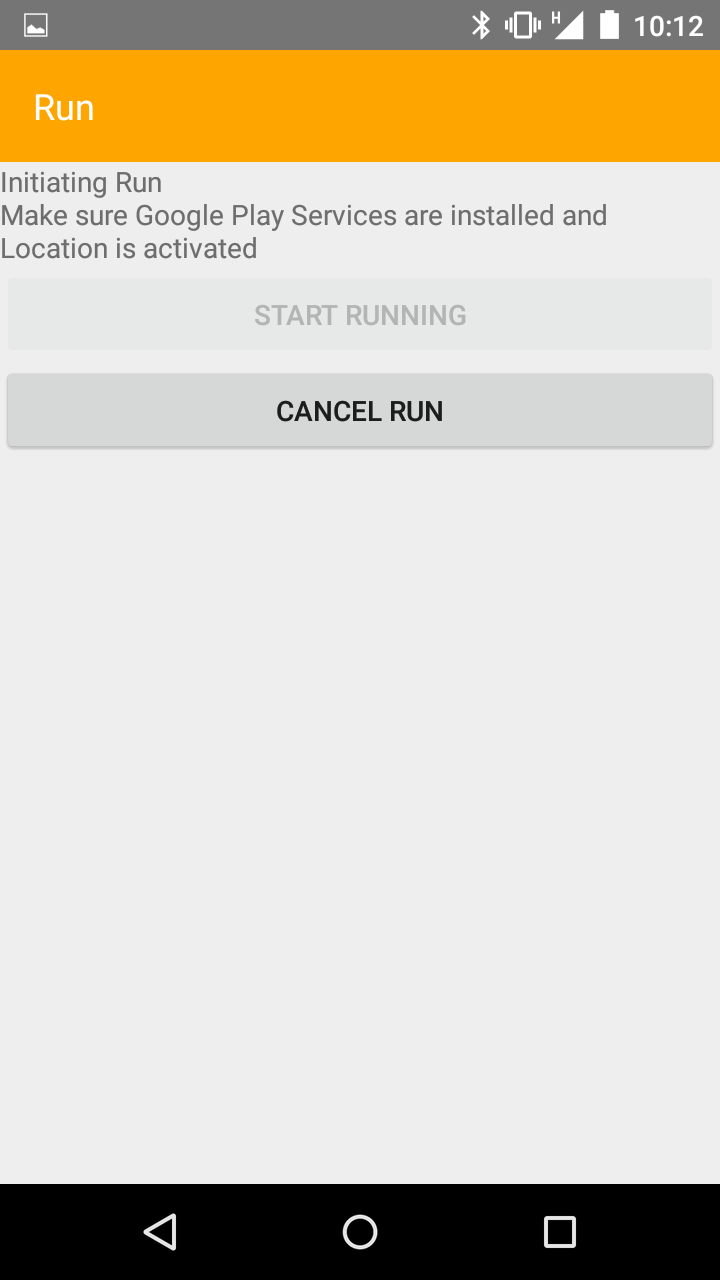
\includegraphics[width=.8\linewidth]{abb/bsp/bsp9}
  \captionof{figure}{Laufinitiierung}
  \label{fig:bsp9}
\end{minipage}
\begin{minipage}{.4\textwidth}
  \centering
  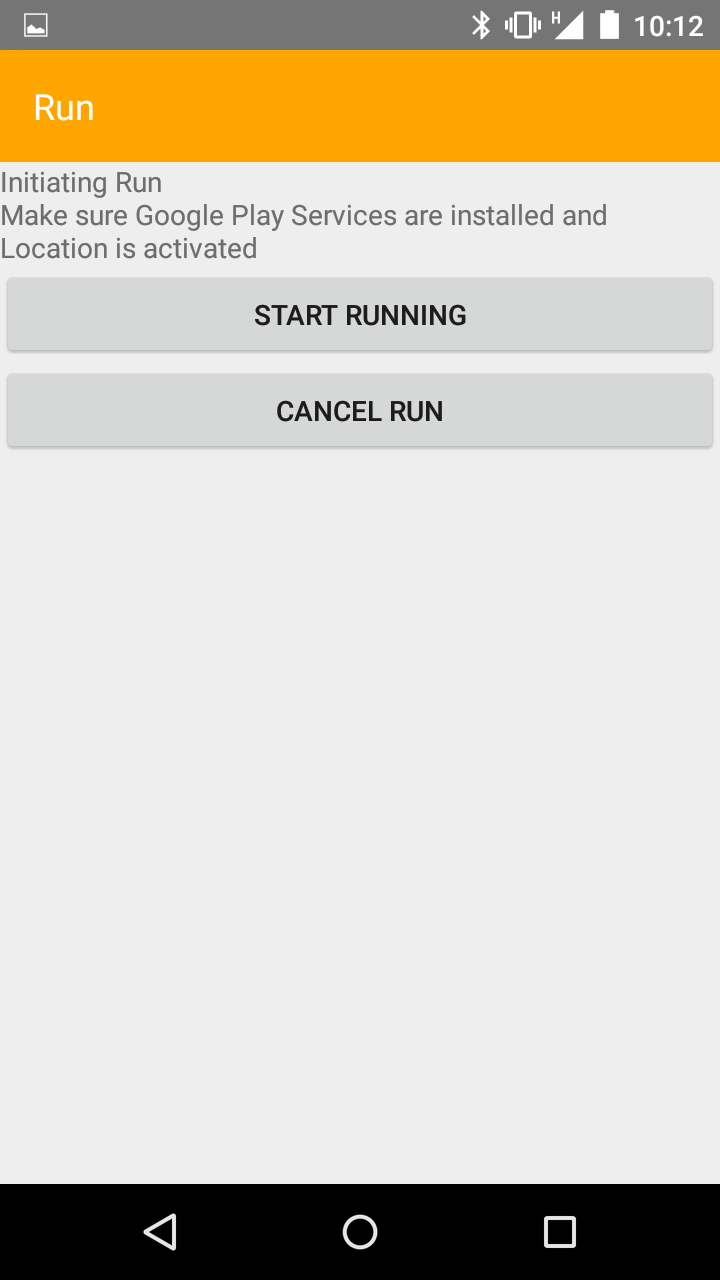
\includegraphics[width=.8\linewidth]{abb/bsp/bsp10}
  \captionof{figure}{Lauf starten}
  \label{fig:bsp10}
\end{minipage}
\end{figure}

Der Lauf wird daraufhin initiert \ref{fig:bsp9} und kann von Eugen gestartet werden, sobald alle nötigen Dateien heruntergeladen sind und der Standortdienst aktiviert ist. \ref{fig:bsp10}

\begin{figure}
\centering
\begin{minipage}{.4\textwidth}
  \centering
  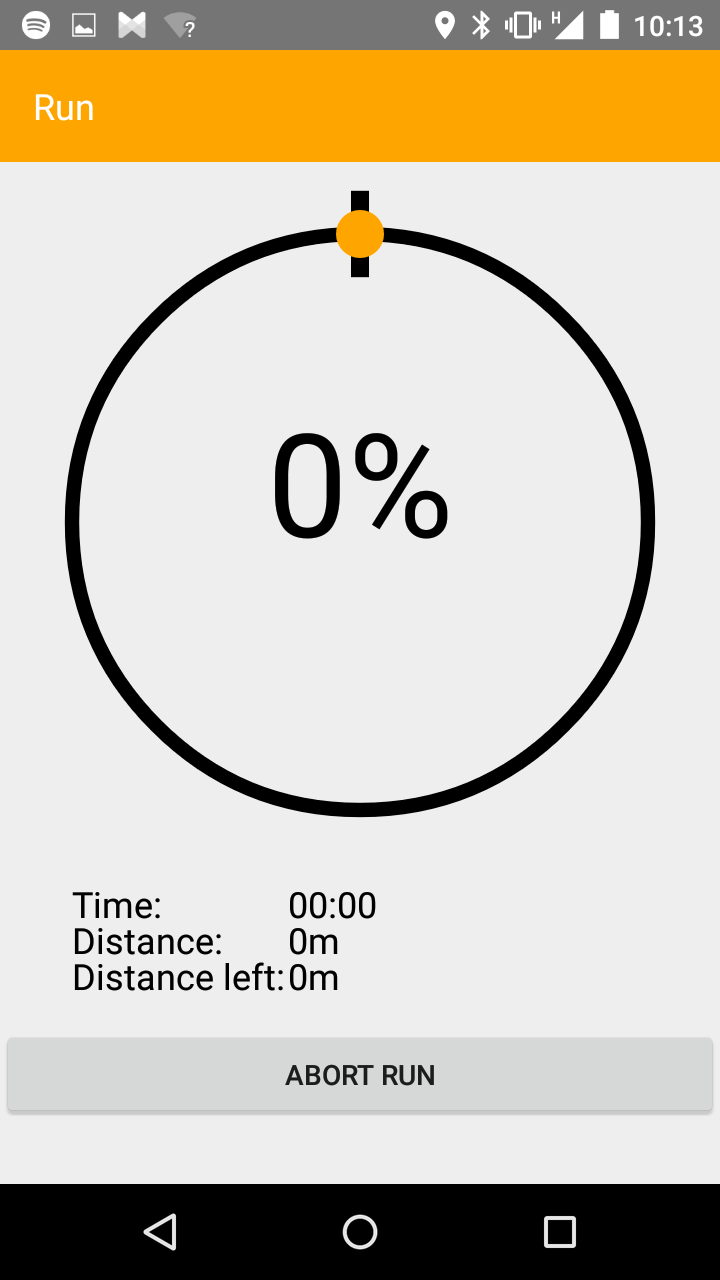
\includegraphics[width=.8\linewidth]{abb/bsp/bsp11}
  \captionof{figure}{Laufanzeige zu Laufbeginn}
  \label{fig:bsp11}
\end{minipage}
\begin{minipage}{.4\textwidth}
  \centering
  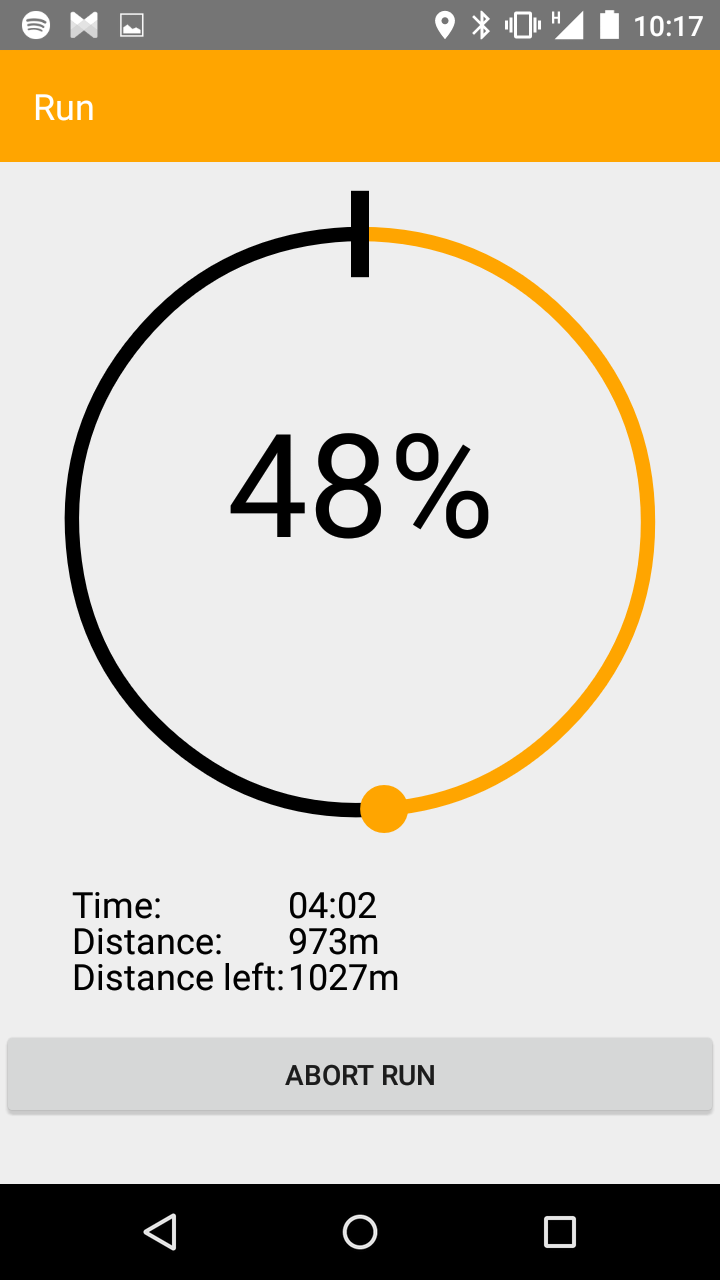
\includegraphics[width=.8\linewidth]{abb/bsp/bsp12}
  \captionof{figure}{Laufanzeige bei halber Strecke}
  \label{fig:bsp12}
\end{minipage}
\end{figure}

Eugen freut sich über die übersichtliche und ansprechende Darstellung des Laufes. Er sieht bildlich seinen Fortschritt und weiß jederzeit, wie weit er noch laufen muss. \ref{fig:bsp11} \ref{fig:bsp12}

\begin{figure}
\centering
\begin{minipage}{.4\textwidth}
  \centering
  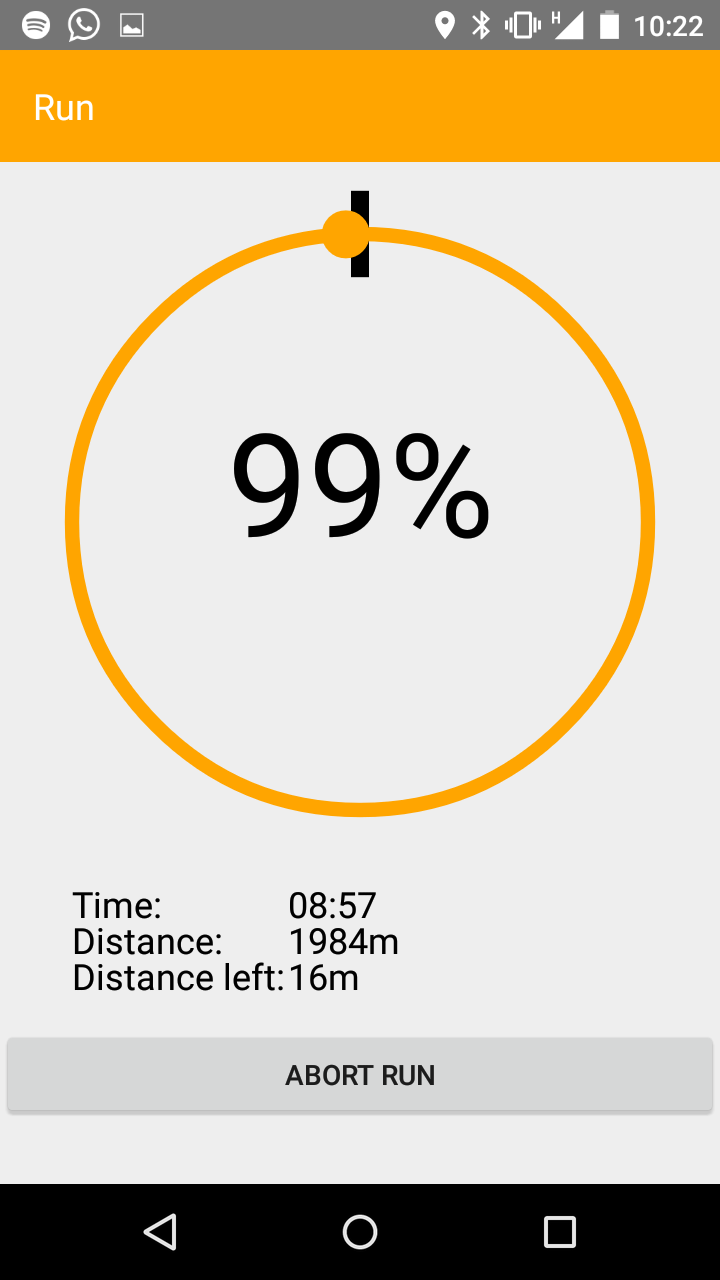
\includegraphics[width=.8\linewidth]{abb/bsp/bsp13}
  \captionof{figure}{Laufanzeige kurz vor dem Ziel}
  \label{fig:bsp13}
\end{minipage}
\begin{minipage}{.4\textwidth}
  \centering
  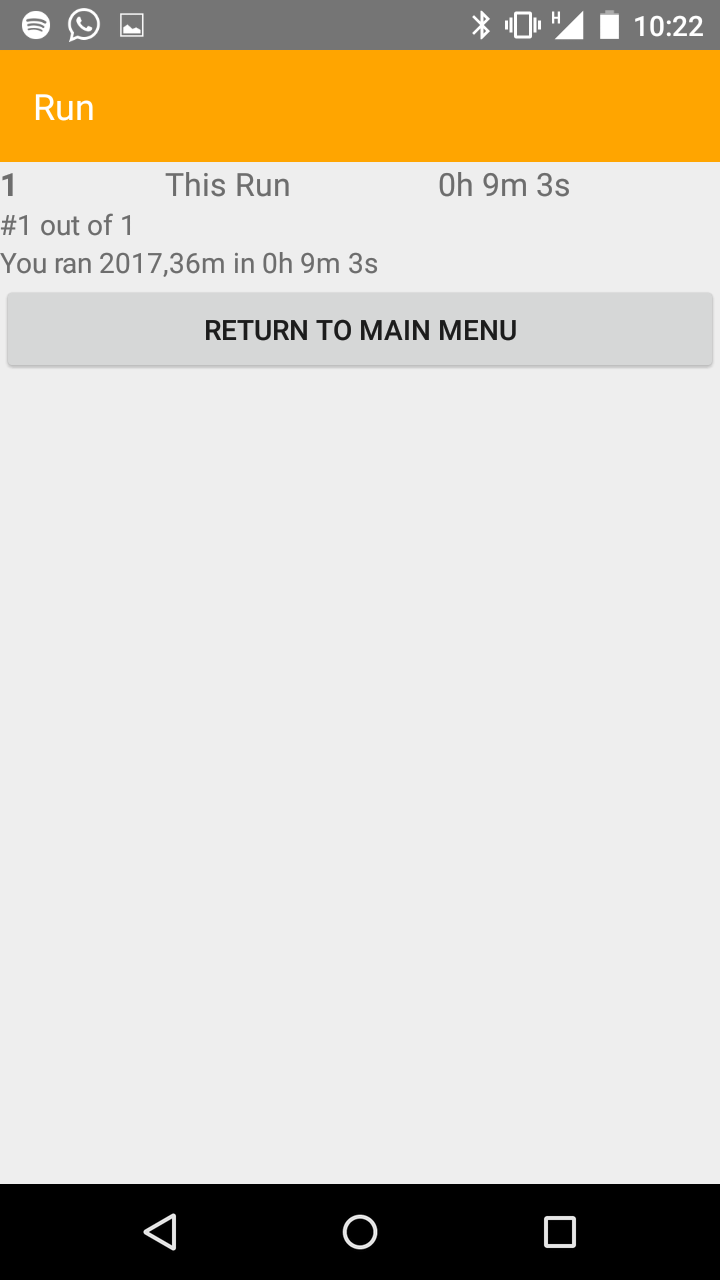
\includegraphics[width=.8\linewidth]{abb/bsp/bsp14}
  \captionof{figure}{Nach Laufende}
  \label{fig:bsp14}
\end{minipage}
\end{figure}

Nach nur neun Minuten ist Eugen im Ziel. Er freut sich, dass alles so reibungslos geklappt hat und dass er heute zum ersten Mal seit Jahren wieder joggen war. \ref{fig:bsp13} \ref{fig:bsp14}

\begin{figure}
\centering
\begin{minipage}{.4\textwidth}
  \centering
  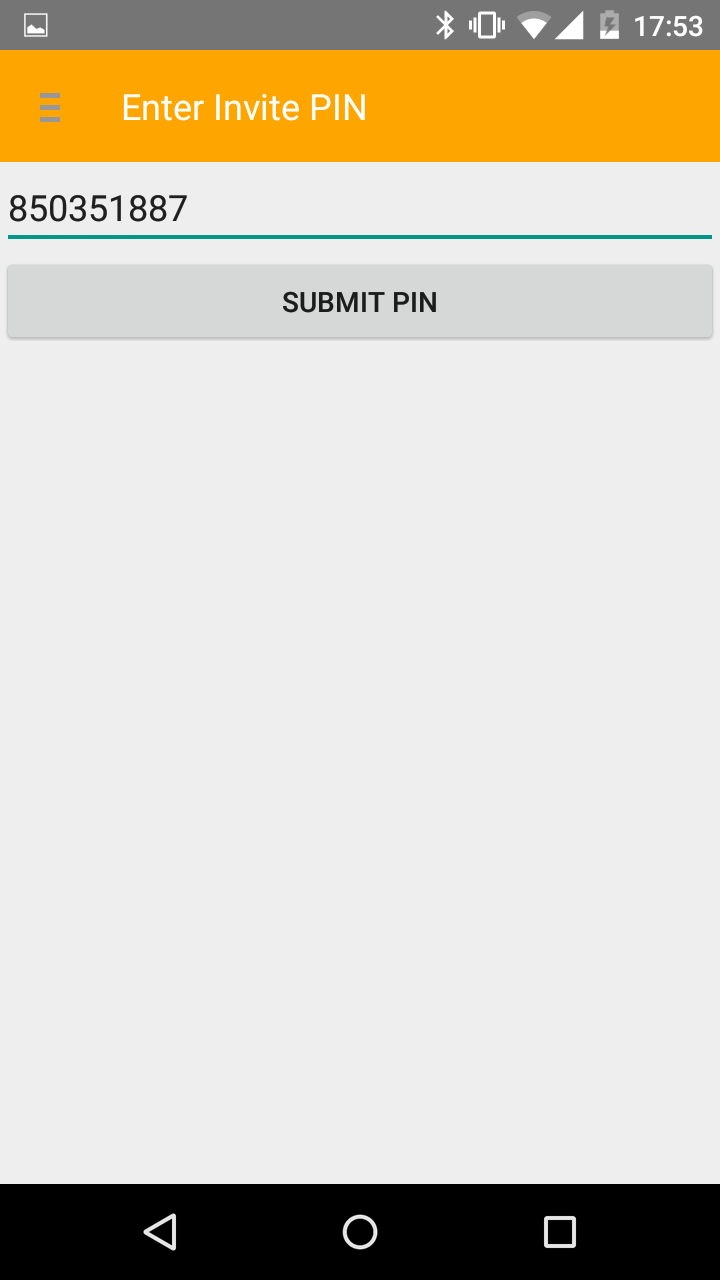
\includegraphics[width=.8\linewidth]{abb/bsp/bsp15}
  \captionof{figure}{Externer Einladung folgen}
  \label{fig:bsp15}
\end{minipage}
\begin{minipage}{.4\textwidth}
  \centering
  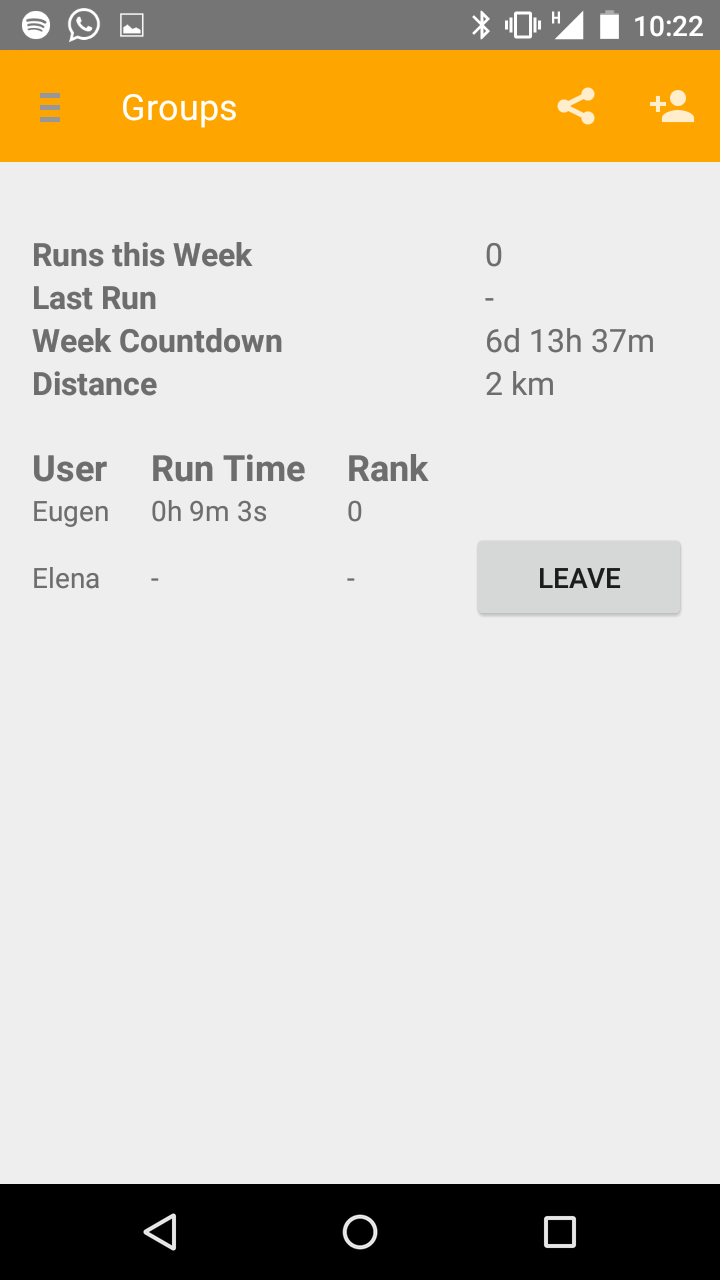
\includegraphics[width=.8\linewidth]{abb/bsp/bsp16}
  \captionof{figure}{Gruppenansicht mit Eugens Lauf}
  \label{fig:bsp16}
\end{minipage}
\end{figure}

Währenddessen sieht Elena Eugens Email. Sie fragt sich, was Gh0strunner ist, will die App aber auf jeden Fall ausprobieren. Nachdem sie sich registriert hat gibt sie die an sie geschickte PIN in das entsprechende Feld ein. \ref{fig:bsp15} Sie sieht die Gruppenübersicht und erkennt, dass Eugen bereits eine Zeit vorgelegt hat. \ref{fig:bsp16} Sofort entscheidet sie sich, ihn herauszufordern.

\begin{figure}
\centering
\begin{minipage}{.4\textwidth}
  \centering
  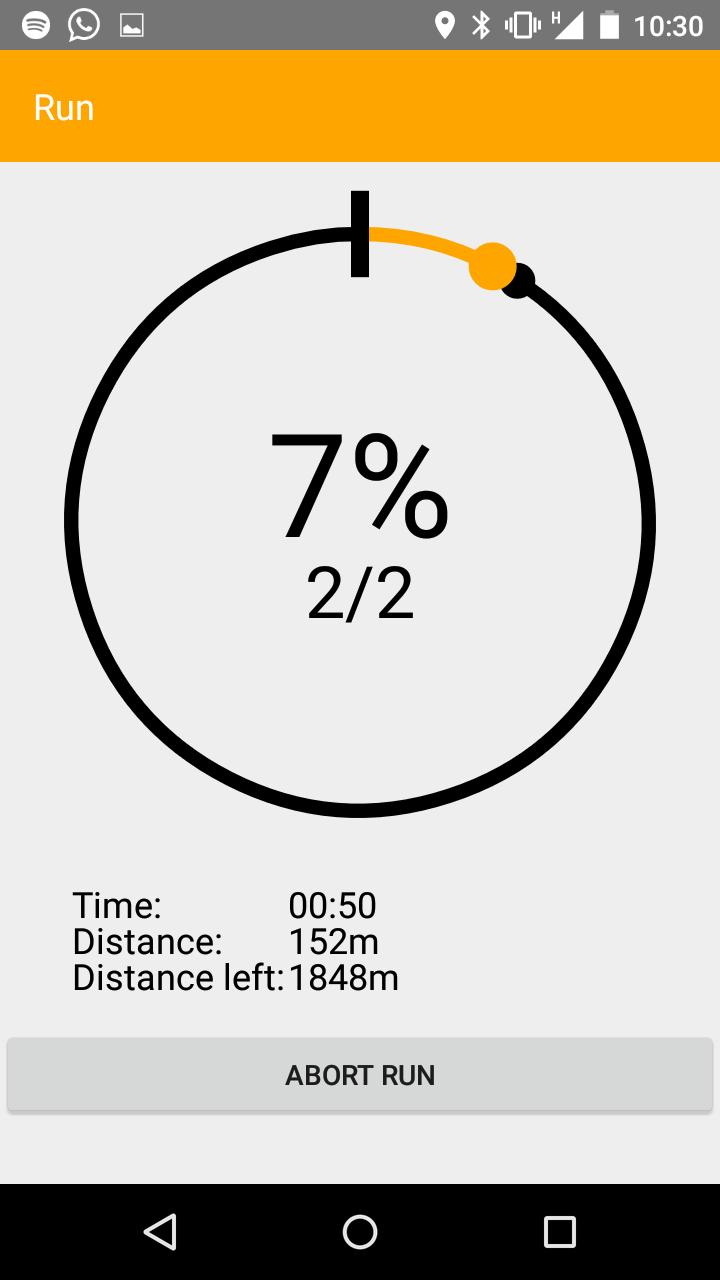
\includegraphics[width=.8\linewidth]{abb/bsp/bsp17}
  \captionof{figure}{Lauf mit Geist und Positionsanzeige}
  \label{fig:bsp17}
\end{minipage}
\begin{minipage}{.4\textwidth}
  \centering
  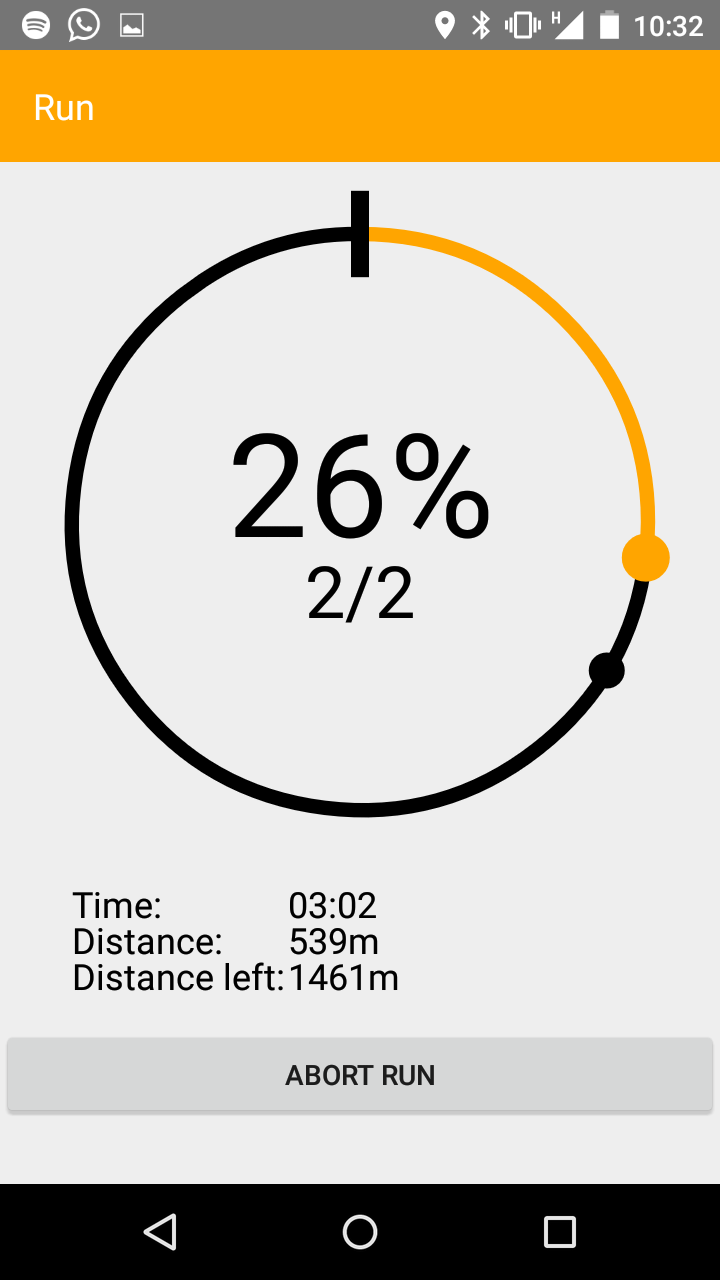
\includegraphics[width=.8\linewidth]{abb/bsp/bsp18}
  \captionof{figure}{Elena liegt hinten}
  \label{fig:bsp18}
\end{minipage}
\end{figure}

Anfangs liegt Elena zurück, sie kann den Geist von Eugen beobachten. \ref{fig:bsp17}. Dieser kann im ersten Viertel seinen Vorsprung immer weiter ausbauen. \ref{fig:bsp18}

\begin{figure}
\centering
\begin{minipage}{.4\textwidth}
  \centering
  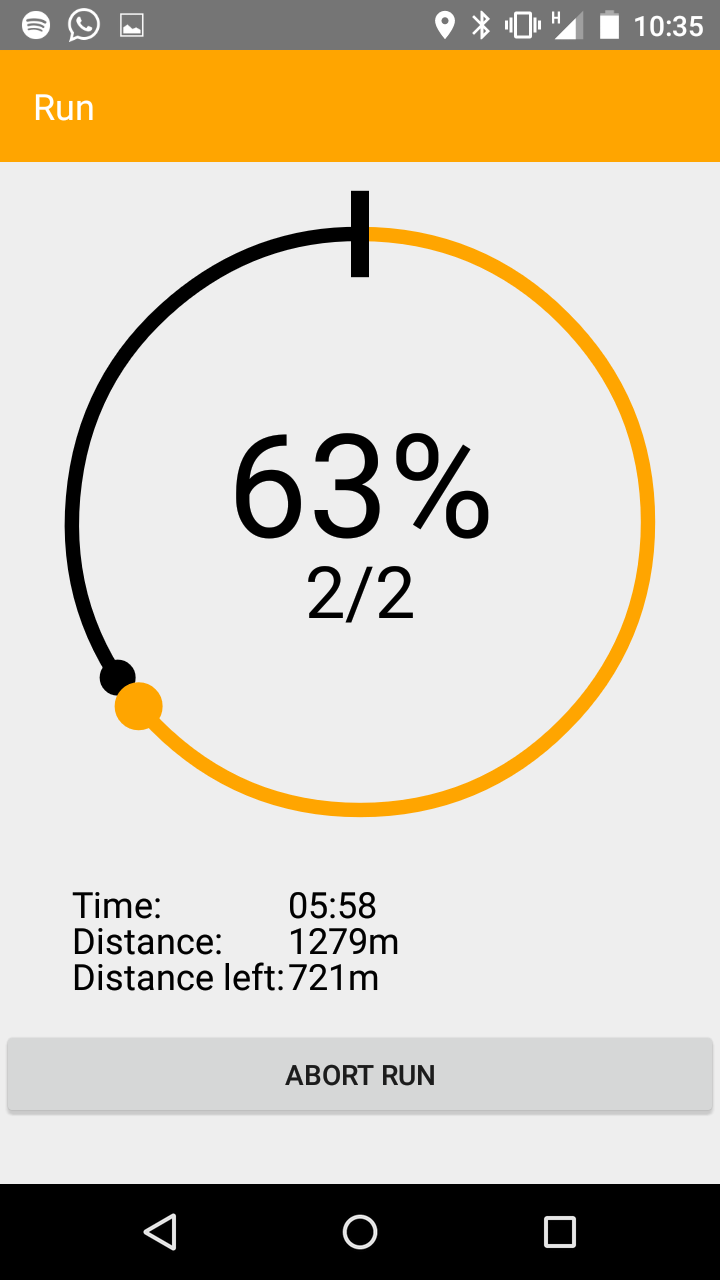
\includegraphics[width=.8\linewidth]{abb/bsp/bsp19}
  \captionof{figure}{Elena versucht aufzuholen}
  \label{fig:bsp19}
\end{minipage}
\begin{minipage}{.4\textwidth}
  \centering
  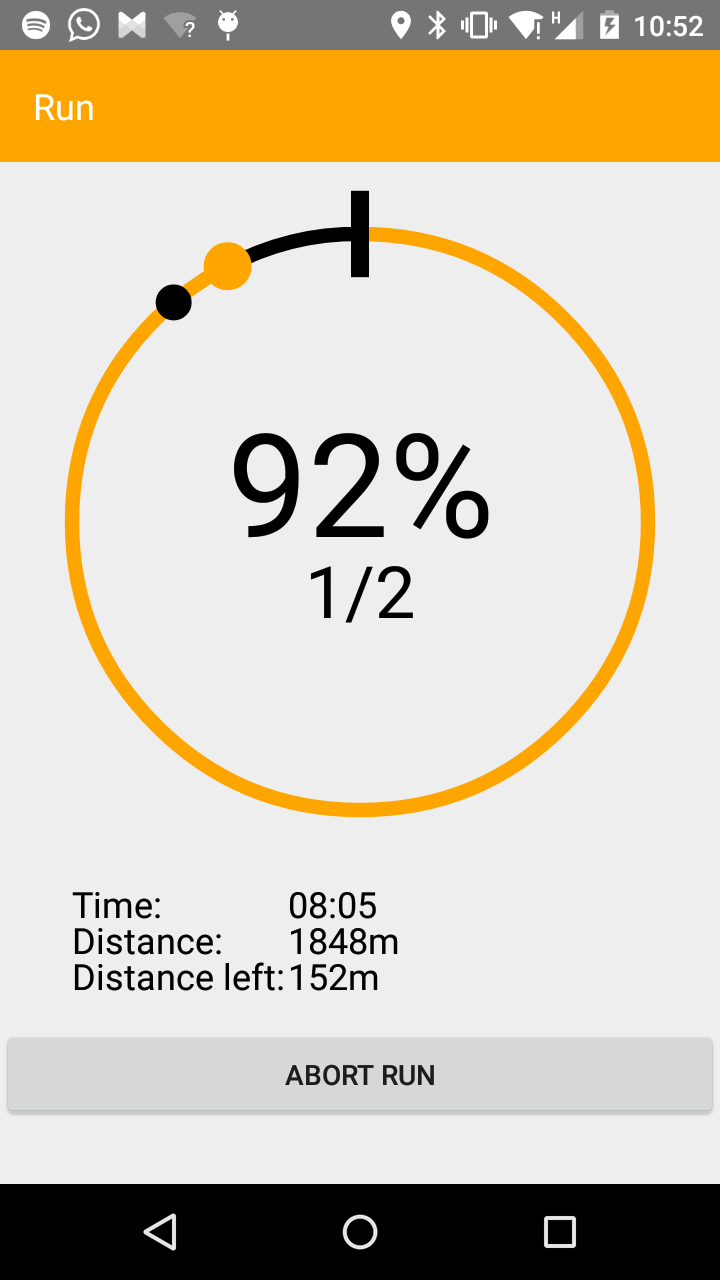
\includegraphics[width=.8\linewidth]{abb/bsp/bsp20}
  \captionof{figure}{Sie hat Eugen überholt}
  \label{fig:bsp20}
\end{minipage}
\end{figure}

Doch Elena strengt sich an, und kann nach zwei Dritteln den Abstand auf Eugen stark verkürzen \ref{fig:bsp19}, um ihn am Ende sogar zu überholen. \ref{fig:bsp20} Sie ist froh, Eugens Geist gesehen zu haben, sonst hätte sie sich mit Sicherheit weniger angestrengt.

\begin{figure}
\centering
\begin{minipage}{.4\textwidth}
  \centering
  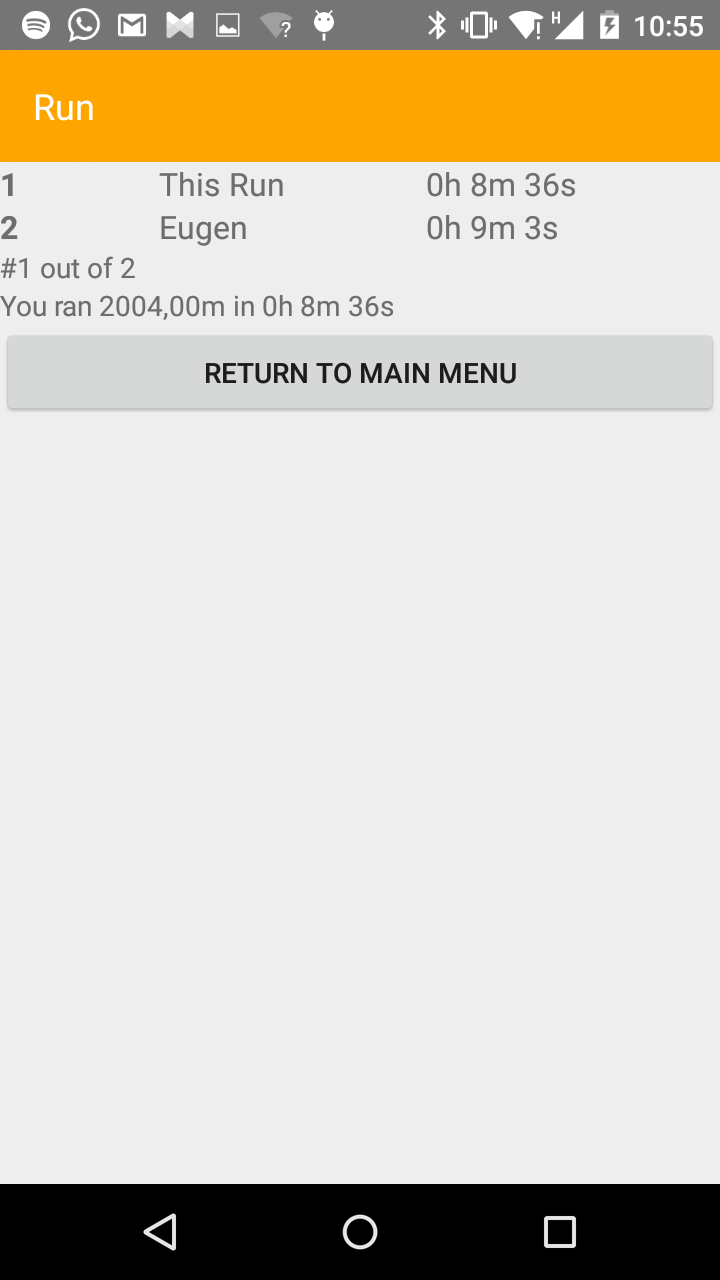
\includegraphics[width=.8\linewidth]{abb/bsp/bsp21}
  \captionof{figure}{Elena gewinnt}
  \label{fig:bsp21}
\end{minipage}
\begin{minipage}{.4\textwidth}
  \centering
  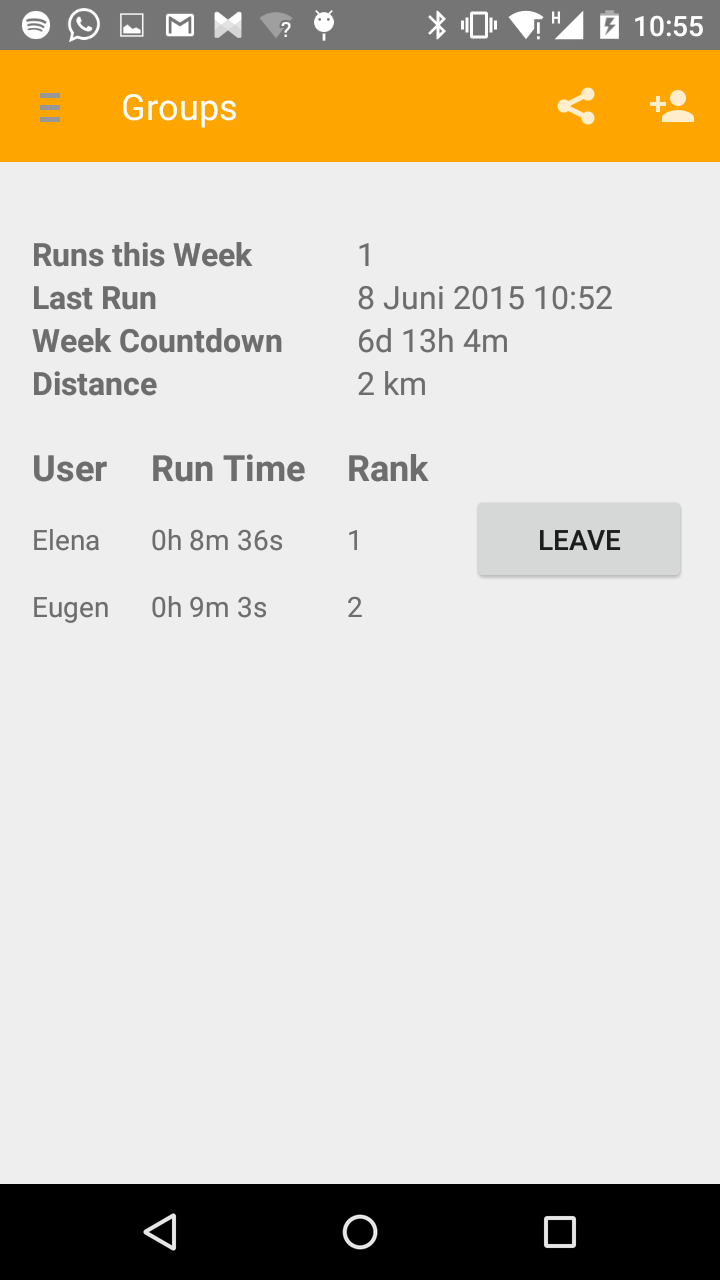
\includegraphics[width=.8\linewidth]{abb/bsp/bsp22}
  \captionof{figure}{Aktualisierte Gruppenansicht}
  \label{fig:bsp22}
\end{minipage}
\end{figure}

Schließlich kann Elena den Lauf abschließen \ref{fig:bsp21}. Eugen hat noch sechs Tage, um seine Zielzeit zu verbessern. \ref{fig:bsp22}

Wir hoffen, mit diesem Beispiel gleichzeitig eine gute Anleitung für die Benutzung der App gegeben zu haben, als auch demonstriert zu haben, wie sie funktioniert.